
% this file is called up by thesis.tex
% content in this file will be fed into the main document

%: ----------------------- introduction file header -----------------------
\begin{savequote}[50mm]
The logic of validation allows us to move between the two limits of dogmatism and skepticism. 
\qauthor{Paul Ricoeur}
\end{savequote}


\chapter{Evaluación}
\label{cha:Validation of the methodology}

% the code below specifies where the figures are stored
\ifpdf
    \graphicspath{{5_experiments_and_results/figures/PNG/}{5_experiments_and_results/figures/PDF/}{5_experiments_and_results/figures/}}
\else
    \graphicspath{{5_experiments_and_results/figures/EPS/}{5_experiments_and_results/figures/}}
\fi


%------------------------------------------------------------------------- 

En este capítulo se evalúa la idoneidad del método propuesto para la evaluación de competencias genéricas. Este capítulo se estructura de la siguiente manera:

\begin{itemize}
	\item En primer lugar se describen las características de los procedimientos que se han utilizado para llevar a cabo la evaluación:
		\begin{itemize}
			\item Publicaciones
			\item Cuestionarios
		\end{itemize}
	\item En segundo lugar se muestran los resultados de la aplicación en cada una de las actividades de aprendizaje para los que se ha implementado el método:
		\begin{itemize}
			\item Wikis: AMW
			\item VLE: SASQL Y EvalCourse
			\item Mundos virtuales: VWQL Y EvalSim
		\end{itemize}
	\item Finalmente se presentan las conclusiones de estas evaluaciones, tanto de los cuestionarios como de las publicaciones.
\end{itemize}

\section{Introducción}

La evaluación del método se ha realizado desde dos perspectivas. Por un lado, cada una de las implementaciones realizadas se ha tratado de mostrar tanto en congresos y revistas de relevancia en el área de las TEL. Mientras que por otro lado, se han realizado cuestionarios y entrevistas a profesionales de la enseñanza para evaluar la idoneidad de los indicadores obtenidos. A continuación se introducen ambos enfoques.

\subsection{Publicaciones}

Durante el desarrollo de este método se ha tratado de publicar en diferentes ámbitos a partir de cada una de sus implementaciones. La evaluación realizada en revistas de ímpacto y conferencias de relevancia son realizadas mediante procesos de \emph{revisión por par doble-ciego}, donde tanto los revisores como los autores son anónimos~\cite{ladron2008revision}. De esta forma se han recibido evaluaciones, opiniones y recomendaciones, que se han ido incorporando a las diferentes implementaciones y al método.

\subsection{Cuestionarios y entrevistas}

En el transcurso de esta tesis se ha presentado en varios foros el trabajo que se va desarrollando. Los profesionales de la educación que han asistido a las presentaciones han participado en cuestionarios de evaluación de la propuesta y han vertido sus opiniones y recomendaciones sobre el método en las entrevistas realizadas. Los profesionales que han participado son profesores universitarios, profesores de primaria y secundaria y personal de MediaWiki España.

% AMW ---------------------------------------------------------------------------------
\section{AMW aplicado a MediaWiki}

El estudio de caso donde se aplica por primera vez AMW se presentó en el \emph{SPEDECE 2012 (Ninth multidisciplinary symposium on the design and evaluation of digital content for education)}~\cite{Balderas:2012} y se amplió en la versión enviada a la revista Computers \& Education en 2015~\footnote{http://www.journals.elsevier.com/computers-and-education/}, pendiente aún de ser publicada.

\subsection{Evaluación}

El estudio de caso en el que se aplicó AMW tuvo lugar en la titulación de \emph{Ingenieria Técnica en Informática de Sistemas},  de la Universidad de Cádiz, en el curso 2011-12. La experiencia fue desarrollada en la asignatura de \emph{Administración de Sistemas Operativos} con 40 estudiantes matriculados. Dentro de las actividades de la asignatura se incluyó el desarrollo de un proyecto en el wiki, que fue evaluado mediante una aproximación mixta con SMW y AMW.

En una primera iteración del \emph{ciclo de contraste de hipótesis} se obtuvieron indicadores cuantitativos, mientras que en la segunda iteración los indicadores que se obtuvieron fueron cualitativos. 
Las dimensiones que se pretendían evaluar fueron las siguientes:

\begin{itemize}
	\item Trabajo en equipo ($M_1$)
	\item Comunicación y la aplicación del conocimiento ($M_2$)
	\item Habilidades individuales ($M_3$)
	\item Capacidad critica ($M_4$)
	\item Entregable final ($M_5$)
\end{itemize}

\subsubsection{Indicadores cuantitativos}

Para la evaluación de competencias en este primer ciclo se decidió partir de indicadores cuantitativos, midiendo en bytes la cantidad de trabajo realizada por cada estudiante en las contribuciones hechas al wiki. Para ela aplicación del método se usó SMW. Los indicadores que se utilizaron fueron los siguientes:

\begin{itemize}
	\item Trabajo en equipo ($M_1$): Ratio de miembros del equipo que contribuyeron en el proyecto wiki.
	\item Comunicación y la aplicación del conocimiento ($M_2$): Ratio de miembros del equipo que contribuyeron al menos a un 20\percentage del conteo final de bytes de la categoría.
	\item Habilidades individuales ($M_3$): contribución en bytes.
	\item Capacidad critica ($M_4$): No considerado
\end{itemize}

\subsubsection{Indicadores cualitativos}

En esta segunda iteración del \emph{ciclo de contraste de hipótesis} se utilizó AMW para obtener indicadores cualitativos. Había numerosos aspectos que se escapaban de la evaluación después de obtener los indicadores cuantitativos y que un análisis cualitativo complementaría. Los indicadores que se utilizaron en este caso para las competencias fueron los siguientes:

\begin{itemize}
	\item Trabajo en equipo ($M_1$): Ratio de miembros del equipo que trabajaron en el mismo criterio técnico.
	\item Comunicación y la aplicación del conocimiento ($M_2$): Media de las notas que los miembros del equipo recibieron.
	\item Habilidades individuales ($M_3$): Media de las notas que cada estudiante recibió.
	\item Capacidad critica ($M_4$): Número de evaluaciones que el estudiante realizó y que fueron posteriormente modificadas por el profesor.
\end{itemize}

\subsubsection{Resumen}

En la tabla~\ref{table:skill-assessed} puede verse una comparativa de los indicadores cuantitativos y cualitativos. Durante el análisis de los indicadores cuantitativos se detectaron pequeños defectos que tuvieron que ser completementados con indicadores cualitativos. 

\begin{table}[h]
\centering
\begin{tabular}{|m{3.1cm}|m{5cm}|m{5cm}|}
\hline
\textbf{Competencia} & \textbf{Indicadores cuantitativos} & \textbf{Indicadores cualitativos}   \\ \hline
\hline
Trabajo en equipo & Ratio de miembros del equipo que contribuyeron a la misma página wiki dentro del proyecto & Ratio de miembros del equipo que trabajaron en el mismo criterio técnico \\
\hline
Comunicación y aplicación del conocimiento & Ratio de miembros del equipo que contribuyeron al menos al 20\percentage del conteo final de bytes de la categoría  & Media de las notas que los miembros del equipo recibieron  \\
\hline
Habilidades individuales  & Contribución en bytes & Media de las notas que el estudiante recibió \\
\hline
Pensamiento  & & Número de evaluaciones que \\
crítico & \emph{No considerado} & el estudiante hizo y fueron \\
 & & modificadas por el profesor  \\
\hline
Entregable final & Manualmente & Manualmente \\
\hline
\end{tabular}
\caption{Resumen de indicadores para cada aproximación.}
\label{table:skill-assessed}
\end{table}

En la competencia de trabajo en equipo, con el enfoque cuantitativo, era muy sencillo para muchos estudiantes conseguir un indicador positivo, ya que por el simple hecho de haber escrito algo en la página era suficiente. Sin embargo, esto no justificaba en sí un trabajo en equipo, sino el haber trabajado algo, aunque fuese poco, en el mismo proyecto. Por ello se planteó el enfoque cualitativo. Al considerarse varios aspectos en un trabajo, y el estar estos aspectos representados en criterios de la rúbrica, el hecho de que dos o más estudiantes tuviesen alguna calificación en un mismo criterio podría considerarse como una evidencia de que esos estudiantes han trabajado en colaboración para alcanzar el objetivo representado en dicho criterio.

Para la competencia de la comunicación y la aplicación del conocimiento se consideró la cantidad de miembros del equipo que contribuyó al menos al 20\percentage de la versión final del wiki en términos de bytes. Este indicador evalúa el nivel de competencia de los equipos de trabajo que contribuyen al éxito del proyecto. Sin embargo, este indicador podía ser confuso. Si un estudiante mueve un trozo de texto considerable el sistema consideraría esta acción como una contribución importante cuando en realidad no lo merece. Incluso un estudiante podría engañar al sistema de pegando texto absurdo y borrándolo después, y así contribuir a unas cifras de trabajo que no serían reales pero que pasarían por alto en un análisis cuantitativo. Por eso, este indicador se complementó con un análisis cualitativo, en el que si un estudiante mueve un trozo de texto de un sitio a otro, quizás pueda obtener una beuan nota en el criterio de la coherencia del texto, pero desde luego no en un criterio específico. En este enfoque cualitativo, a partir de la media de todas las calificaciones de todas las contribuciones de los miembros del equipo se mide cómo han aplicado los estudiantes el conocimiento y cómo se han comunicado para este fin.

Para las competencias de las habilidades individuales nos encontramos ante la misma situación. Medir en bytes el trabajo de los profesores te aporta un dato cuantitativo válido, pero que necesita un análisis cualitativo que tenga en cuenta posibles situaciones que se tendrían en cuenta con el enfoque cuantitativo. Con la media de las calificaciones de las contribuciones realizadas individualmente por cada estudiante se complementa la evaluación de esta competencia.

Para el pensamiento crítico se tiene en cuenta sólo el aspecto cualitativo. Los estudiantes disponen del conocimiento para realizar la evaluación del trabajo de sus compañeros. Los estudiantes evaluados pueden reclamar una evaluación recibida si no están de acuerdo con la misma. En ese caso es el profesor el que se encarga de la revisión, y si modifica la nota, el alumno evaluador será penalizado en esta competencia.

\subsection{Resultados}
La experiencia constaba de las tres fases que fueron introducidas en el capítulo anterior:

\begin{description}
\item[1. Desarrollo del trabajo en el wiki]

Esta etapa se inició con un seminario donde los estudiantes aprendieron cómo debían trabajar colaborativamente en un wiki basado en MediaWiki. Después, los estudiantes se dividieron en doce grupos de tres miembros y dos grupos de dos miembros. Cada grupo tuvo que escribir la documentación de su proyecto en una sola página wiki. Dado que uno de los objetivos de la asignatura era desarrollar una experiencia de \emph{evaluación auténtica}, el cometido del proyecto era la planificación y gestión del proceso de migración real de un sistema de información de la empresa. Los estudiantes fueron los responsables de la planificación y la gestión de su asignación, la coordinación de sus tareas y del trabajo en colaboración. El wiki está disponible públicamente~\footnote{http://wikis.uca.es/wikiASO/}, y en seis semanas de los estudiantes crearon más de 1.400 ediciones en los 14 proyectos que participaron en la asignatura. Como guía de esta experiencia, mostraremos los resultados obtenidos por los cuatro grupos de tres miembros de la tabla~\ref {tab:AmwGroupsMembers}.

\begin{table}[h]
\centering
\begin{tabular}{|c|c|}
\hline
\textbf{Project ($P_i$)} & \textbf{Members ($U_i$)}   \\ \hline
\hline
 $P_1$ & $U_7$, $U_8$, $U_9$  \\ \hline
 $P_4$ & $U_{13}$, $U_{14}$, $U_{15}$  \\ \hline
 $P_7$ & $U_4$, $U_5$, $U_6$  \\ \hline
 $P_{13}$ & $U_1$, $U_2$, $U_3$  \\ \hline
\end{tabular}
\caption{Grupos de ejemplo y sus miembros.}
\label{tab:AmwGroupsMembers}
\end{table}

\item[2. Evaluación de los estudiantes]

Esta fase comenzó con un seminario. Los estudiantes aprendieron cómo evaluar contribuciones al wiki mediante el uso de AMW. Tras ello, los estudiantes realizaron 412 evaluaciones cualitativas de contribuciones al wiki. Este proceso proporcionó a los estudiantes información crítica sobre su trabajo. Los estudiantes también pudieron replicar una evaluación si no estaban de acuerdo con la misma.

\item[3. Revisión del profesor]

El profesor tuvo que resolver las réplicas. Esta información se utilizó más tarde para evaluar el pensamiento crítico.

\end{description}

AMW se utilizó para evaluar el desempeño de los estudiantes en varios indicadores relacionados con el trabajo en equipo. Indicadores como la coordinación para desempeñar tareas y su desempeño de manera colaborativa. Además, se fomento el pensamiento crítico de los estudiantes motivándoles a revisar formalmente el trabajo de sus compañeros para que su nota no se bajase.

A continuación en cada subsección se explica cómo se evaluaron las competencias para cada subdimensión. Esta propuesta se basa en el programa de la asignatura. Dependiendo de la configuración de las tareas específicas del wiki y de la actividad a desarrollar, el profesor podría utilizar estos indicadores como proponemos, adaptarlos a la evaluación de otras habilidades, o incluso definir sus indicadores.

\subsubsection{Indicador del trabajo en equipo ($M_1$)}

\paragraph*{Aproximación cuantitativa}

Mediante el uso de SMW se pudo comprobar como todos los miembros de cada equipo, en menor o mayor medida habían participado en la páginas wikis de sus proyectos. Este indicador se descartó, ya que una vez analizado lo único que podíamos saber era si los estudiantes habían contribuido al proyecto, pero el hecho de haber contribuido al mismo proyecto no es necesariamente una evidencia de haber trabajado en equipo. Por tanto, este indicador se redifinió mediante la aproximación cualitativa.

\paragraph*{Aproximación cualitativa}

Esta calificación mide la habilidad de un equipo para trabajar colaborativamente y era compartida por todos los miembros del equipo ($U_i$) de cada proyecto ($P_i$). Esta dimensión recogía los criterios en los que fue evaluado cada $U_i$ en la página de su proyecto. Consideramos que un $U_i$ ha contribuido en un criterio de un proyecto si ha sido evaluado en ese criterio en alguna de sus contribuciones.

De esta forma, dos o más estudiantes colaboraron si fueron evaluados en el mismo criterio. Si dos miembros del equipo fueron evaluados en criterios complementarios, ello no implicaba colaboración. Bajo esta premisa sólo se consideraron los criterios técnicos, que están relacionados con las partes de la tarea en la que los estudiantes en realidad colaboraron. La colaboración en criterios transversales como la escritura o la coherencia no se consideraron ($D_{11}$-$D_{17}$).

En la tabla~\ref{table:13-project-grades} se muestran los criterios evaluados para cada miembro del proyecto $P_{13}$. Mientras que $U_1$ fue evaluado en cinco criterios, $U_2$ y $U_3$ sólo fueron evaluados de uno. Los criterios \emph{servidor físico} ($D_4$) , \emph{red} ($D_6$) , \emph{PCs} ($D_7$) , \emph{Gantt} ($D_9$) y \emph{presupuesto} ($D_10$) sólo fueron trabajados por un miembro del equipo ($U_1$). El único criterio trabajado por más de un miembro del equipo fue $D_8$, que fue trabajado por $U_1$ y $U_2$. Así que, bajo nuestra propuesta, $U_1$ y $U_2$ trabajaron colaborativamente, pero $U_3$ no.

\begin{table}[h]
\centering
\begin{tabular}{|c|c|c|c|c|c|c|c|c|c|c|l|}
\hline
\textbf{Estudiante} & \textbf{$D_1$} & \textbf{$D_2$} & \textbf{$D_3$} & \textbf{$D_4$} & \textbf{$D_5$} & \textbf{$D_6$} & \textbf{$D_7$} & \textbf{$D_8$} & \textbf{$D_9$} & \textbf{$D_{10}$} & \textbf{Collaboración} \\ \hline
\hline
$U_1$ &   &   &   & 1 &   &     & 1   & \textbf{1}  & 1  & 1  & \textbf{sí (en $D_8$ con $U_2$)} \\ \hline
$U_2$ &   &   &   &    &   &     &      & \textbf{1}    &      &       & \textbf{sí (en $D_8$ con $U_1$)} \\ \hline
$U_3$ &   &   &   &    &   & 1  &     &      &      &       & \textbf{no} \\ \hline
% \hline
% \hline
% Sum &   &   &   & 1 &   & 1  & 1   & \textbf{2}  & 1  & 1  & \textbf{2 out of 3} \\ \hline
% \hline\multicolumn{13}{|c|}{\textbf{1 out of 3 $\rightarrow$ 33.3\% $\rightarrow$ \underline{3.33 out of 10}}} \\ \hline
\end{tabular}
\caption{Grading of collaborative work ($M_1$) in the $P_{13}$ project.}
\label{table:13-project-grades}
\end{table}

Finalmente, la calificación del grupo en esta dimensión se calculaba con la fórmula~\ref{math:m1}. 

\begin{equation}
    \textbf{$M_1 = CTM/TM$}
    \label{math:m1}
\end{equation}

En dicha fórmula participan las siguientes variables:

\begin{itemize}	
	\item \emph{CTM (collaborative team members}: número de miembros del equipo que trabajaron colaborativamente.
	\item \emph{TM (team members)}: número de miembros que componen el equipo.
\end{itemize} 

La calificación $M_1$ para el proyecto $P_{13}$ fue de 6,66 sobre 10, ya que dos de los tres miembros trabajaron colaborativamente.

\subsubsection{Indicador de las habilidades de comunicación y la aplicación del conocimiento ($M_2$)}

\paragraph*{Aproximación cuantitativa}

En este enfoque se considera la cantidad de miembros de cada equipo que habían contribuido al menos a un 20\percentage del trabajo realizado en la página del wiki medido en bytes (para equipos de tres estudiantes). En la figura~\ref{fig:smw-p13} puede verse una gráfica de la distribución del trabajo, mostrándose el ratio total de bytes contribuidos por cada estudiante del proyecto $P_{13}$. $U_1$ (verde) contribuyó con un 38,2\percentage, $U_2$ (rojo) con un 27,2\percentage y $U_3$ (azul) con un 34,7\percentage. Al estar más o menos balanceada consideramos que ellos trabajaron colaborativamente.

\begin{figure}
	\centering
	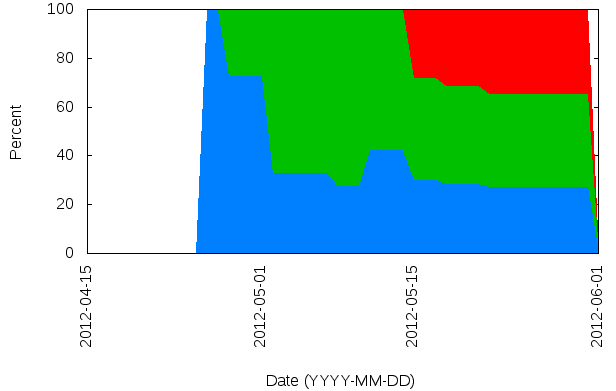
\includegraphics[width=8cm]{smw-work-distribution-p13.png}
	\caption{Distribución del trabajo de los miembros del proyecto $P_{13}$.}
	\label{fig:smw-p13}
\end{figure}

\paragraph*{Aproximación cualitativa}

Esta calificación medía la habilidad para aplicar el conocimiento en situaciónes prácticas y la habilidad para comunicarse con otros miembros del equipo. La calificación de este indicador también era compartida por todos los miembros del equipo ($U_i$). Se calcula como la media de las notas que cada miembro del equipo recibió. Este indicador evaluaba la eficacia de los equipo de trabajo que contribuyen al éxito del proyecto. Notas medias en las contribuciones pueden significar pobres contribuciones al wiki o que algunas contribuciones obtuvieron buenas calificaciones y otras malas, evidenciando una comunicación deficiente entre los miembros del equipo o un escaso grado de compromiso con el equipo.

La media de todas las calificaciones dadas a los criterios de cada contribución a los miembros de cada equipo en el proyecto se calcula mediante la fórmula~\ref{math:m2}.

\begin{equation}
    \textbf{$M_2 = SRA_G/NRA_G$}
    \label{math:m2}
\end{equation}

En dicha fórmula participan las siguientes variables:
\begin{itemize}	
	\item \emph{$SRA_G$ (sum of received assessments)}: suma de las calificaciones recibidas para todas las contribuciones del proyecto.
	\item \emph{$NRA_G$ (number of received assessments)}: número de evaluaciones recibidas.
\end{itemize} 

\begin{table}[h]
\centering
\begin{tabular}{|c|r|r|r|r|r|r|r|r|r|r|r|r|r|}
\hline
\textbf{Estudiante} & \textbf{$D_1$} & \textbf{$D_2$} & \textbf{$D_3$} & \textbf{$D_4$} & \textbf{$D_5$} & \textbf{$D_6$} & \textbf{$D_7$} & \textbf{$D_8$} & \textbf{$D_9$} & \textbf{$D_{10}$} & \textbf{$D_{11}$} &  \textbf{$SRA_G$ } & \textbf{$NRA_G$ } \\ \hline
\hline
$U_4$ & 15  & 13  & 7  & 26 & 22 & 34  & 30 & 6   & 25  & 37 & 89  & \textbf{304} & \textbf{40} \\ \hline
$U_5$ &      &      &     & 26 & 8   &      &      &      &  18 &      & 17 &  \textbf{69}  & \textbf{8} \\ \hline
$U_6$ &     &  8    &    &  25 & 9  &     &   7   &  8   &      &  8  &  133 & \textbf{198} & \textbf{26} \\ \hline
\hline
\hline
\multicolumn{12}{|r|}{\textbf{Suma}} & 571 &  74 \\ \hline
\multicolumn{12}{|r|}{\textbf{Media}} & \multicolumn{2}{|c|}{\textbf{7.71}} \\ \hline
\end{tabular}
\caption{($M_2$) para el proyecto $P_{7}$.}
\label{table:7-project-peers-grades}
\end{table}

\begin{table}[h]
\centering
\begin{tabular}{|c|r|r|r|r|r|r|r|r|r|r|r|r|r|}
\hline
\textbf{Estudiante} & \textbf{$D_1$} & \textbf{$D_2$} & \textbf{$D_3$} & \textbf{$D_4$} & \textbf{$D_5$} & \textbf{$D_6$} & \textbf{$D_7$} & \textbf{$D_8$} & \textbf{$D_9$} & \textbf{$D_{10}$} & \textbf{$D_{11}$} &  \textbf{$SRA_G$ } & \textbf{$NRA_G$ } \\ \hline
\hline
$U_{13}$ &   &   &   & 24 &      & 15  & 7   & 7   & 8   & 47  & 98  & \textbf{206} & \textbf{27} \\ \hline
$U_{14}$ &   &   &   & 26 & 8   &      &      &      &  27 &      & 10 &  \textbf{37}  & \textbf{4} \\ \hline
$U_{15}$ & 22 &  46 & 21   &  40 & 17  & 5 & 94 &  5   & 6  &  20  &  123 & \textbf{399} & \textbf{64} \\ \hline
\hline
\hline
\multicolumn{12}{|r|}{\textbf{Suma}} & 642 &  95 \\ \hline
\multicolumn{12}{|r|}{\textbf{Media}} & \multicolumn{2}{|c|}{\textbf{6.75}} \\ \hline
\end{tabular}
\caption{$M_2$  para el proyecto $P_{4}$.}
\label{table:4-project-peers-grades}
\end{table}

% Dejo la parte cuantitativa??
%Para la evaluación cuantitativa se consideró la cantidad de miembros del equipo que contribuyeron al menos a un 20\percentage de los bytes de la versión final del wiki (para equipos de tres estudiantes). En la figura~\ref{} puede verse una gráfica de la distribución del trabajo, mostrándose el ratio total de bytes contribuidos por cada estudiante del proyecto $P_{13}$. $U_1$ (verde) contribuyó con un 38,2\percentage, $U_2$ (rojo) con un 27,2\percentage y $U_3$ (azul) con un 34,7\percentage. Al estar más o menos balanceada consideramos que ellos trabajaron colaborativamente.

\subsubsection{Indicador de habilidades individuales ($M_3$)}

\paragraph*{Aproximación cuantitativa}

bla bla bla

\paragraph*{Aproximación cualitativa}

Esta dimensión evalúa la capacidad para producir y mantener la calidad del proyecto. Es una habilidad individual, y se calcula por separado para cada miembro del equipo ($U_i$). El grado en esta dimensión es el promedio de las calificaciones recibidas para cada alumno, expresado en la fórmula~\ref{math:m3}.

\begin{equation}
    \textbf{$M_3 = SRA_S/NRA_S$}
    \label{math:m3}
\end{equation}

En dicha fórmula participan las siguientes variables:
\begin{itemize}	
	\item \emph{$SRA_S$ (sum of received assessments by the student)}: suma de las calificaciones recibidas para las contribuciones del estudiante.
	\item \emph{$NRA_S$ (number of received assessments by the student)}: número de evaluaciones recibidas por el estudiante.
\end{itemize} 

El promedio de las calificaciones asignadas a las contribuciones de cada estudiante del proyecto $P_4$ ($U_{13}$, $U_{14}$, $U_{15}$) y del proyecto $P_{13}$ ($U_1$, $U_2$, $U_3$) puede verse en la tabla~\ref{table:project-individual-grades}. Bajo nuestro enfoque, los miembros de $P_{13}$ tuvieron calificaciones similares. Pero en $P_4$ puede verse un constraste, ya que $U_{14}$ hizo buenas aportaciones, mientras que $U_{15}$ no contribuyó a la calidad del proyecto.

\begin{table}[h]
\centering
\begin{tabular}{|c|c|r|r|r|r|r|r|r|r|r|r|r|r|r|r|}
\hline
\textbf{$P_i$} & \textbf{$U_i$} & \textbf{$D_1$} & \textbf{$D_2$} & \textbf{$D_3$} & \textbf{$D_4$} & \textbf{$D_5$} & \textbf{$D_6$} & \textbf{$D_7$} & \textbf{$D_8$} & \textbf{$D_9$} & \textbf{$D_{10}$} & \textbf{$D_{11}$} &  \textbf{$SRA_G$ } & \textbf{$NRA_G$ } & \textbf{$M_3$} \\ \hline
\hline
\multirow{3}{*}{$P_{13}$} & $U_1$ &   &   &   & 7 &   &     & 15   & 13  & 16  & 40  & 24 & 115 & 15 & 7.67 \\
 & $U_2$ &   &   &   &    &   &     &      & 8    &      &       &     & 8    & 1   & 8.00 \\
 & $U_3$ &   &   &   &    &   & 14  &     &      &      &       & 15 &  29 & 4   & 7.25  \\ \hline
 & $U_{13}$ &   &   &   & 24 &      & 15  & 7   & 7   & 8   & 47  & 98  & \textbf{206} & \textbf{27} & 7.62 \\ 
 & $U_{14}$ &   &   &   & 26 & 8   &      &      &      &  27 &      & 10 &  \textbf{37}  & \textbf{4} & 9.25 \\ 
\multirow{-3}{*}{$P_{4}$} & $U_{15}$ & 22 &  46 & 21   &  40 & 17  & 5 & 94 &  5   & 6  &  20  &  123 & \textbf{399} & \textbf{64} & 6.23 \\ \hline
\end{tabular}
\caption{($M_3$) para los miembros de $P_{4}$ y $P_{13}$.}
\label{table:project-individual-grades}
\end{table}

% Cuantitativo?

\subsubsection{Indicador del pensamiento crítico ($M_4$)}

\paragraph*{Aproximación cuantitativa}

bla bla bla

\paragraph*{Aproximación cualitativa}

Como se ha comentado anteriormente, AMW permitió a los estudiantes replicar si estabán en desacuerdo con una evaluación recibida. Esas réplicas se reportaron al supervisor para resolverlos. En caso de que el profesor aceptase una réplica, la calificación se modificaba. Pero este proceso tiene otra parte: los estudiantes recibieron instrucciones claras sobre la tarea de evaluación, siendo un proceso formativo que tenía reflejo en su calificación. Entonces, podíamos utilizar esta información como un indicador de la habilidad para \emph{interpretar, analizar y evaluar el trabajo de sus compañeros}. En particular, hemos utilizado dos indicadores: el número de evaluaciones realizadas por cada estudiante y la cantidad de ellos que el profesor modificó (podían tener su origen en réplicas del estudiante evaluado o en revisiones al azar realizadas por el profesor). No fue nuestro caso, pero si había diferentes evaluaciones en una misma contribución, la diferencia entre ellos podría ser también un indicador de competencia.

La fórmula que se utilizó fue~\ref{math:m4}. Se considera que todos los estudiantes comenzaron con 10 puntos en esta dimensión, y perdieron 2,5 de ellos por cada evaluación que hicieron  y que fue modificado por el profesor, hasta un mínimo de 0 puntos. De hecho, cada estudiante hizo 10 evaluaciones, por lo que consideramos que deberían haber hecho no más del 20\percentage de las evaluaciones erróneas para aprobar esta parte de la nota. En nuestro caso de estudio, tuvimos 412 evaluación, y 27 de ellas (6\percentage) se replicaron (el profesor sólo revisó las evaluaciones replicadas). Sólo 10 de ellas (37\percentage) fueron aceptadas. En cuanto a los estudiantes, sólo uno tuvo 3 réplicas a sus evaluacones aceptadas. El resto de ellos tenía 2, 1 o ninguno. En la tabla~\ref{table:students-grade-replies} pueden verse las evaluaciones realizadas por los miembros de $P_{13}$ que fueron respondidas. $U_1$ y $U_2$ recibieron una réplica que fue aceptada ($AR$) cada uno, mientras que $U_3 $ no tuvo ninguna.

\begin{equation}
    \textbf{$M_4 = 10 - 2.5 * AR$}
    \label{math:m4}
\end{equation}

\begin{table}[h]
\centering
\begin{tabular}{|c|c|c|c|}
\hline
\textbf{Students} & \textbf{Received replies} & \textbf{Accepted replies} & \textbf{$M_4$}  \\ \hline
\hline
 $U_1$ & 2 & 1 & 7.50  \\ \hline
 $U_2$ & 1 & 1 & 7.50 \\ \hline
 $U_3$ & 0 & 0 & 10.00  \\ \hline
\end{tabular}
\caption{($M_4$) para los miembros del proyecto $P_{13}$.}
\label{table:students-grade-replies}
\end{table}

\subsubsection{Entregable final ($M_5$)}

Para la calificación fina se tomó el trabajo final del wiki, donde se valoraron todos los requisitos que se esperaban del trabajo. En nuestro enfoque, cada $P_i$ tuvo una calificación entre 0-10. Esta fue la calificación dada por el profesor una vez se ha llegado a la fecha límite. La calificación fue la misma para todos los miembros del equipo ($U_i$), ya que todos ellos (como equipo) son responsables del resultado final del proyecto. Los proyectos fueron evaluados usando la rúbrica indica en el cuadro~\ref{table:project-rubric-supervisor}. Hay dos categorías de criterios en las rúbricas:

\begin{itemize}
\item Criterios específicos: atributos desde $D_1$ a  $D_{10}$, que se refieren a aspectos específicos del trabajo. 
\item Criterios transversales: atributos desde $D_{11}$ a  $D_{17}$, que se refieren a aspectos transversales del trabajo: coherencia, correcto uso del formato wiki, ... etc.
\end{itemize}

\begin{table}[h]
\centering
\begin{tabular}{|c|l|r|r|}
\hline
\textbf{Item} & \textbf{Criterios}  & \textbf{Peso}  & \textbf{Nota ($P_{13}$) }   \\ \hline
\hline
 $D_1$ & Justificación &  2.00 & 2.00 \\ \hline
 $D_2$ & Centro de datos anterior &   0.25 & 0.25 \\ \hline 
 $D_3$ & Centro de datos nuevo &    0.25 & 0.25 \\ \hline 
 $D_4$ & Servidor físico &    0.25 & 0.25  \\ \hline
 $D_5$ & Servidor virtual &    0.25 & 0.25  \\ \hline 
 $D_6$ & Red &    0.50 & 0.50  \\ \hline 
 $D_7$ & PCs &  0.40 & 0.40  \\ \hline 
 $D_8$ & Formación &    0.25 & 0.25  \\ \hline 
 $D_9$ & Diagrama de Gantt &    0.40  & 0.20  \\ \hline
 $D_{10}$ & Presupuesto &   0.40  & 0.40 \\ \hline
 $D_{11}$ & Escritura &   0.30  & 0.30 \\ \hline
 $D_{12}$ & Coherencia &   3.00  & 2.40 \\ \hline
 $D_{13}$ & Referencias &    0.25  & 0.00 \\ \hline
 $D_{14}$ & Formato wiki &    0.50  & 0.50 \\ \hline
 $D_{15}$ & Aplicación de conceptos teóricos &    1.00  & 0.50 \\ \hline
 $D_{16}$ & Información extra &    1.00  & 0.00 \\ \hline
 $D_{17}$ & Plagio &    -10.00  & -0.00 \\ \hline
 \hline
 \multicolumn{2}{|c|}{\textbf{Suma}} & \textbf{(Máx.) 10.00} & \textbf{8.45} \\ \hline
\end{tabular}
\caption{Calificaciones dadas por el profesor al proyecto $P_{13}$.}
% \caption{Grades the supervisor gave to the $P_{13}$ project using the rubric for the final version of the wiki pages.}
\label{table:project-rubric-supervisor}
\end{table}

A modo de ejemplo, la cuarta columna de la tabla muestra las calificaciones que el supervisor le dio a los criterios del proyecto $P_{13}$. Este proyecto fue calificado con un 8,45 puntos sobre 10. Esta evaluación cualitativa manual realizada por el supervisor es escalable, ya que cada grupo solo tiene una versión definitiva de su página wiki.

\subsection{Discusión} % Dejar? Eran resultados ...

Junto con el estudio de caso, varias comparaciones entre el enfoque cuantitativo previo y la cualitativa implementada en esta experiencia han sido desplegados. Un resumen sobre las ventajas del enfoque cualitativo se muestra a continuación:

\begin{itemize}
\item El enfoque cualitativo permite un análisis más fino de grano de trabajo colaborativo en comparación con los que en el experimento cuantitativo anterior.
\item Además, este análisis también puede detectar a los estudiantes que colaboran con un objetivo común en las diferentes páginas del wiki de un mismo proyecto.
\item Este enfoque permite la detección de las contribuciones que copiar, borrar y pegar de grandes fragmentos de texto sin tener que mejorar la página wiki, lo que podría tener una buena medición cuantitativa inmerecida.
\item Las contribuciones a otros proyectos se incluyen en la calificación individual de los estudiantes, mientras que estas contribuciones fueron de grano grueso en cuenta en el enfoque cuantitativo anterior.
\item La capacidad de los estudiantes para ser crítico es entrenado y evaluado por el proceso de respuesta.
\end{itemize}

Mientras que las principales desventajas son las siguientes:

\begin {itemize}
\item La función de selección debe ser cuidadosamente elegido, por lo que las evaluaciones se llevan a cabo en las contribuciones significativas.
\item Revisión de todas las evaluaciones de los compañeros y auto realizados por los estudiantes sigue siendo una tarea difícilmente escalable para el supervisor. Por lo tanto, algunas evaluaciones pobres pueden no detectados por el supervisor si no se informan, ni eligieron al azar para ser revisado.
\end {itemize}

En líneas generales, los estudiantes tuvieron un buen desempeño en la tarea. En la tabla~\ref{table:summary-theory} puede verse como solo 3 estudiantes no aprobaron el proyecto ($6.98\%$). Sin embargo, 37 estudiantes ($86.04\%$) tuvieron una buena calificación, más de 7 sobre 10. Los estudiantes llevaron a cabo tareasde análisis crítico mediante la evaluación del trabajo de sus compañeros. Así, obtuvieron retroalimentación y evidencias para cada evaluación recibida.

\begin{table}[h]
\centering
\begin{tabular}{|c|c|r|}
\hline
\textbf{Notas} & \textbf{Estudiantes} & \textbf{Ratio}   \\ \hline
\hline
 [9-10] & 16 & 37.21\% ~ \\ \hline
 [8-9) & 10 & 23.25\% ~ \\ \hline
 [7-8) & 11 & 25.58\% ~ \\ \hline
 [6-7) & 3 & 6.98\% ~ \\ \hline
 [5-6) & 0 & 0\% ~ \\ \hline
 [0-5) & 3 & 6.98\% ~ \\ \hline
\end{tabular}
\caption{Resumen de calificaciónes finales de los estudiantes}
\label{table:summary-theory}
\end{table}

%It is interesting to underline that the best peer-assessed grades were received by those students who were assessed fewest times. In particular there are only two students that had a grade average of 10, and they only had 1 and 3 assessments respectively. In fact, the following maximum one was 9.25, an average obtained by two students, both with 4 assessments. This was probably because they wrote large and very polished contributions. When their peers assessed them, they gave a very good grade because of the amount and quality of the information added. The only issue with these students is that they did not probably work collaboratively, and as a consequence had a lower grade in this dimension. This makes sense: if a student focuses on doing very few and large editions their mates can have problems to collaborate with them: they log in the wiki, contributes (a nice piece of text) and leave. So any issue of coherence with the rest of the project, or rewriting to adapt to change must be done by other team members (or it could even remain undone in the final version of the wiki page).


%Finally, 21 out of the 412 assessments (5\%) were self-assessment. The 85.71\% of these grades were between 8 and 9, and only one was below 5. After manually checking some of them, we have to acknowledge that were well assessed, although they weren't as severe with themselves as with their peers. Perhaps in a future case study every self-assessment should be automatically noticed to the supervisor to be checked and, eventually, could be considered an evidence of self-critical skill.

%Additionally, we could also detect the group organization, i.e. the roles adopted by each member. This was done by aggregating the criteria that each group member worked. This way we can identify groups where each member focused on different criteria. This is not necessarily bad if the final version of the wiki page is good. But in case it was not, it would be an evidence of a problem in group internal dynamics: probably each member did their work and nobody cared of relating individual parts to produce a coherent deliverable in the wiki. We could check the talk pages (both of the project pages and users ones) to see if they communicated and, in that case, the role that each member played.


% EVALCOURSE ---------------------------------------------------------------------------------
\section{EvalCourse aplicado a entornos de apredizaje virtual}

Los estudios de caso que se presentan en este capítulo fueron publicados en la revista~\emph{International Journal of Engineering Education, Special issue on Innovative Methods of Teaching Engineering}~\cite{Balderas:2015}, después de haber sido invitados a extender un primer trabajo presentado en el~\emph{4th International Workshop on Software Engineering for E-learning (ISELEAR’13)}~\cite{balderas2013generative}.

\subsection{Evaluación}

Los estudios de caso en los que se aplicó EvalCourse tuvieron lugar en dos asignaturas de la titulación de \emph{Ingenieria Informática}, de la Universidad de Cádiz, en el curso 2012/13. La evaluación del curso se realizó de forma manual, y después se aplicó EvalCourse para evaluar a los estudiantes en las competencias de liderazgo, habilidades interpersonales y el pensamiento crítico.

\subsubsection{Extracción de indicadores del foro}

El primero de los casos de estudio tuvo lugar en la asignatura de \emph{Procesadores de Lenguajes II} y que tenía 36 estudiantes matriculados. Era una asignatura obligatoria, que tenía lugar en el primer semestre del quinto (y último) curso. Durante el semestre, los estudiantes tuvieron que trabajar en pequeños equipos de dos o tres miembros. Cada equipo del curso tenía un foro para la comunicación interna. Este foro se utilizó para evaluar dos competencias: habilidades interpersonales y liderazgo.

En primer lugar, como indicador de las habilidades interpersonales de cada estudiante se calculó el total de intervenciones en el foro. El coordinador del curso animó a sus estudiantes a participar en el foro del equipo, ya que debía ser su herramienta de comunicación interna. Un estudiante que tenía tres o más intervenciones en el foro tendría una buena calificación. En segundo lugar, como indicador de liderazgo se consideró los debates que los estudiantes iniciaron en el foro. Un estudiante que inició dos o más debates tuvo una calificación positiva en la competencia de liderazgo.

\paragraph*{Análisis}

Sólo 18 de los 36 estudiantes del curso participaron en los foros. No se puede determinar que los estudiantes que no participaron en el foro no posean las competencias, lo único que podemos afirmar es que no demostraron su desempeño en estas competencias a través de esta actividad. Los resultados de haber aplicado EvalCourse pueden verse en el listado de la tabla~\ref{tab:EvcEvaluacionListadoForo1}. Pocos estudiantes obtuvieron una calificación positiva en estas competencias, habiendo varios estudiantes que destacan sobre el resto. Estos datos se exportaron a una hoja de cálculo y se genero la figura~\ref{fig:EvcEvaluacionTartaForo1}. En resumen, consideramos que los estudiantes, a pesar de que sabían que debían utilizar el foro para la comunicación entre los miembros del equipo, no lo hicieron en su mayoría.

\begin{table}
	\centering
	\caption{Listado de intervenciones de los estudiante en el foro.}
	\label{tab:EvcEvaluacionListadoForo1}
	\begin{tabular}{|c|l|c|c|c|}
		\hline
		id & username & Debate- & Debate- & Total  \\
			&		&	starter	& participation		&		\\
		\hline
		\hline
		43 &	S2 &	0 &	1 &	 1 \\
		44 &	S3 &	3 &	4 &	 7 \\
		45 &	S4 &	2 &	2 &	 4 \\
		46 &	S5 &	0 &	1 &	 1 \\
		48 &	S7 &	4 &	3 &	 7 \\
		50 &	S9 &	6 &	8 &	 14 \\
		51 &	S10 &	1 &	1 &	 2 \\
		53 &	S12 &	0 &	1 &	 1 \\
		55 &	S14 &	1 &	1 &	 2 \\
		59 &	S18 &	1 &	2 &	 3 \\
		60 &	S19 &	2 &	0 &	 2 \\
		61 &	S20 &	0 &	2 &	 2 \\
		62 &	S21 &	0 &	1 &	 1 \\
		67 &	S26 &	0 &	1 &	 1 \\
		70 &	S29 &	0 &	1 &	 1 \\
		71 &	S30 &	2 &	1 &	 3 \\
		75 &	S34 &	1 &	5 &	 6 \\
		78 &	S37 &	2 &	4 &	 6 \\
		\hline
	\end{tabular}
\end{table}

\begin{figure}
	\centering
	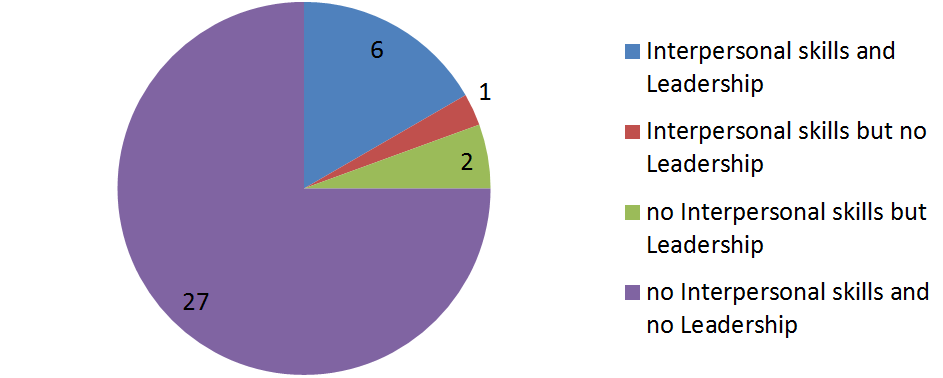
\includegraphics[width=12cm]{EvcForo1.png}
	\caption{Resumen del desempeño de los estudiantes en el foro en las dos competencias.}
	\label{fig:EvcEvaluacionTartaForo1}
\end{figure}

A pesar de esto, de manera informal sí se observó que los estudiantes con calificaciones positivas en ambas competencias realmente tuvieron un buen desempeño de dichas competencias en la asignatura. Por tanto, pudimos decir que los indicadores elegidos parecían ser verdaderas evidencias del nivel de competencia de los estudiantes. Probablemente el hecho de que el varlos dado a la participación en el foro en la calificación global de la asignatura fuera sólo de un 2,5\percentage no animó a los estudiantes a no utilizar en exclusiva sus habituales métodos de comunicación (Whatsapp, correo electronico, reuniones en el pasillo, etc.).

También se utilizó EvalCourse para analizar la interacción entre los estudiantes. La idea era localizar interacciones que quizás estuviese más interesadas en mejorar sus resultados que en la mera comunicación. Se detectaron evidencias de interacciones fraudulentas entre dos estudiantes cuando se podía ver que ellos sólo estaban interesados en hablar entre ellos dos y no habían interactuado con ningún otro compañero. Con el código SASQL mostrado en la consulta~\ref{code:interaction1} se obtuvo la interacción que hubo en el foro. Los resultados se pueden ver en la figura~\ref{fig:EvcEvaluacionInteraccionForo2}.


\begin{lstlisting}[caption=Código SASQL para extraer datos sobre la interacción en el foro ,label=code:interaction1,numbers=left, captionpos=b, morekeywords={Evidence,get, students, show, milestones, participation, access, in, assignment, forum, campus, workshop, interaction}]
Evidence forum_interaction: 
	get students
	show interaction
	in forum.
\end{lstlisting}

\begin{figure}
	\centering
	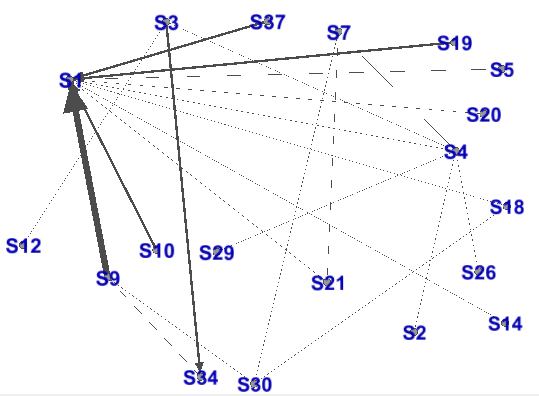
\includegraphics[width=12cm]{EvcForo2.png}
	\caption{Graph of students' interaction in forum case study.}
	\label{fig:EvcEvaluacionInteraccionForo2}
\end{figure}

Concluímos que gran parte de la interacción del foro se debía a mensajes de respuesta al profesor (S1). Esto hecho es un indicio de que en muchos casos la interacción de los estudiantes con el foro es más debida a cuestiones que los estudiantes realizan al profesor para que les aclaren algunas de las intrucciones proporcionadas en el propio foro que al uso del foro como herramienta del grupo.

\subsubsection{Extracción de indicadores del taller}

El segundo estudio de caso que se analizó se desarrolló en la asignatura de Programación Funcional, en la que había 19 estudiantes matriculados. Esta es una asignatura optativa que tiene lugar también en el segundo semestre del quinto (y último) curso. Los estudiantes tuvieron que trabajar en cuatro talleres a lo largo del curso. En Moodle, un taller es un entregable que, conforme a las intrucciones del profesor, puede ser evaluado por otro u otros estudiantes o auto-evaluado. Los estudiantes debían entregar una tarea en un taller habilitado para cada tema antes de la fecha límite fijada en la actividad. Tras la fecha de entrega, el profesor proporcionaba la solución a la tarea, de manera que cada tarea fuera evaluada por dos compañeros de manera aleatoria y por el propio estudiante. A final de curso, se calculó la media de las calificaciones de todos los talleres. Esta calificación era el 30\percentage de la nota de la asignatura, siendo obligatoria una buena calificación para aprobar la asignatura. El profesor de la asignatura tenía que evaluar el pensamiento crítico de sus estudiantes. Para ello, utilizó como indicador para cada tarea la diferencia entre la media de las calificaciones dadas por cada compañero con respecto a la calificación que se asignó el propio estudiante. Cada estudiante evaluaba su propio trabajo antes de saber la calificación que le habían dado sus compañeros.

El grado de validez del indicador proporcionado por EvalCourse dependerá del profesor, que si lo considera oportuno, podrá contrastar o complementar el indicador con otros actividades de aprendizaje. Al igual que los estudiantes deben haber sido instruídos para realizar el trabajo que se les pedia, deben ser capaces de evaluar el trabajo de sus compañeros, argumentando sus criterios, sus razones y sus evidencias.

\paragraph*{Análisis}

A partir del código mostrado en la consulta~\ref{code:EvcWorkshop1}, se obtiene el listado~\ref{tab:EvcWorkshop1} con los indicadores que se utilizaron para evaluar a los estudiantes en la competencia del pensamiento crítico (en un rango de 0 a 10). En la figura~\ref{fig:EvcWorkshop1} se muestra un grafo con la diferencia entre sus auto-calificaciones y las otorgadas por sus compañeros. Este grafo se genero a partir de la iimportación de los indicadores a una hoja de cálculo. En él, se detecta fácilmente a dos estudiantes que se auto-asignaron una calificación inferior a la que le dieron sus compañeros.

\begin{lstlisting}[caption=Extracción evaluaciones realizadas en los talleres ,label=code:EvcWorkshop1,numbers=left, captionpos=b, morekeywords={Evidence,get, students, show, milestones, evaluations, participation, access, in, assignment, forum, campus, between, and, workshop, interaction}]
Evidence workshop_critical: 
	get students
	show evaluations
	in workshop.
\end{lstlisting}

\begin{table}
	\centering
	\caption{Desempeño de los estudiantes en la competencia de la autocrítca.}
	\label{tab:EvcWorkshop1}
	\begin{tabular}{|l|c|c|c|}
		\hline
		username & Peer-grade & Self-grade & Mean-diff \\
		\hline
		\hline
			Stud3 & 5.26 & 5.56 & 0.3 \\
			Stud6 & 6.22 & 7.06 & 0.94 \\
			Stud7 & 5.92 & 7.44 & 1.52 \\
			Stud8 & 7.62 & 8.03 & 0.60 \\
			Stud9 & 9.38 & 9.33 & 0.57 \\
			Stud10 & 7.39 & 8.14 & 0.75 \\
			Stud11 & 5.24 & 5.64 & 0.62 \\
			Stud12 & 7.30 & 6.80 & 0.83 \\
			Stud13 & 8.06 & 7.92 & 0.55 \\
			Stud14 & 9.92 & 9.86 & 0.22 \\
			Stud15 & 5.12 & 6.00 & 1.43 \\
			Stud16 & 7.85 & 7.06 & 0.79 \\
			Stud17 & 9.00 & 8.97 & 0.75 \\
			Stud18 & 6.29 & 7.31 & 1.01 \\
			Stud22 & 7.16 & 8.20 & 1.03 \\
			Stud25 & 8.61 & 8.72 & 0.22 \\
			Stud28 & 8.14 & 8.08 & 0.47 \\
			Stud30 & 9.54 & 9.44 & 0.23 \\
		\hline
	\end{tabular}
\end{table}

\begin{figure}
	\centering
	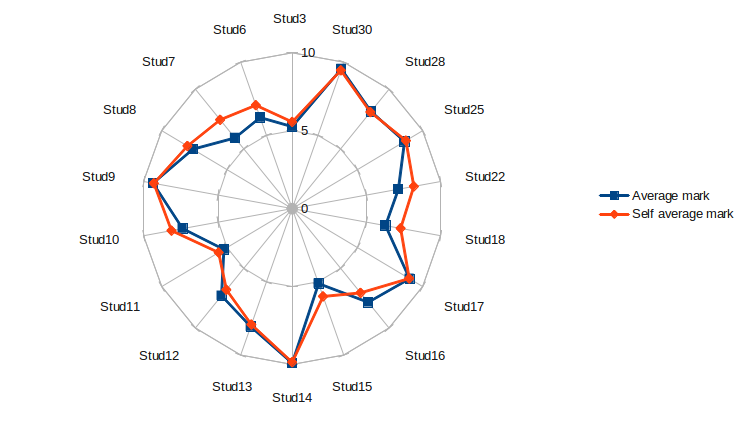
\includegraphics[width=12cm]{EvcWorkshop1.png}
	\caption{Grafo que muestra las diferentes calificaciones que se autoasignaron los estudiantes y la que les dieron sus compañeros.}
	\label{fig:EvcWorkshop1}
\end{figure}

Se puede decir que no hubo muchas diferencias en las calificaciones. Esto es un buen indicador, ya que la mayor parte de los estudiantes que tuvieron una diferencia grande en las primeras calificaciones, corrigieron esta desviación en las siguientes evaluaciones. Aunque también hay estudiantes que hicieron buenas auto-evaluaciones desde el principio, como se puede comprobar viendo la última columna de la tabla~\ref{tab:EvcWorkshop1}. En ella se representa la diferencia media de las calificaciones que recibieron y que se autoasignaron.

En este punto el profesor tuvo que decidir sobre la validez del indicador. Y en caso afirmativo, cuál seria el límite entre una valoración positiva y una negativa. Gracias a que el grupo era pequeño, el profesor podía comparar el comportamiento real observado durante el curso con los resultados del indicador, confirmando que había mucha similitud entre ambas calificaicones. De hecho, el límite positivo se estableció con una media de $0,5$ puntos o menos. Mientras que una valoración negativa se dejó para aquellos cuya diferencia era superior a $1$. Con estos resultados se obtuvo la siguiente distribución (provocando una distribución de campana).

\begin{itemize}
\item Si la diferencia media está entre $0$ y $0,5$, esto era un indicador positivo del desempeño de la competencia de la autocritica. (5 estudiantes).
\item Si la diferencia media está entre $0,5$ y $1$, los estudiantes mostraron un nivel medio de la competencia (9 estudiantes).
\item If the mean difference of the averages is $1$ or higher, esto era un indicador negativo del desempeño de la competencia de la autocritica (4 estudiantes).
\end{itemize}

Por supuesto, se necesitan más estudios para determinar la validez de los resultados de EvalCourse como indicadores de la competencia. Sin embargo, en nuestro caso, pudimos decir que la informaicón fue de utilidad para justificar la evaluación de los estudiantes.

\subsection{Resultados}

Morbi at augue sapien. Duis tempus quam vitae velit interdum ultricies. Vivamus laoreet lacinia elit sit amet vehicula. Ut congue diam ac magna hendrerit sed fermentum justo lacinia. Curabitur vel odio neque, quis consequat mi. Proin lobortis justo quis enim fermentum accumsan sagittis ipsum imperdiet. Proin sem felis, laoreet placerat egestas id, fringilla id mauris. Pellentesque a nisi sit amet leo consectetur gravida nec et dui. Curabitur quis hendrerit augue. Etiam sed dui nec tortor convallis fringilla. Proin tempor mattis diam nec egestas. Quisque condimentum elementum lacus ac porta.

% EVALSIM ---------------------------------------------------------------------------------
\section{EvalSim aplicado a los mundos virtuales}

Morbi at augue sapien. Duis tempus quam vitae velit interdum ultricies. Vivamus laoreet lacinia elit sit amet vehicula. Ut congue diam ac magna hendrerit sed fermentum justo lacinia. Curabitur vel odio neque, quis consequat mi. Proin lobortis justo quis enim fermentum accumsan sagittis ipsum imperdiet. Proin sem felis, laoreet placerat egestas id, fringilla id mauris. Pellentesque a nisi sit amet leo consectetur gravida nec et dui. Curabitur quis hendrerit augue. Etiam sed dui nec tortor convallis fringilla. Proin tempor mattis diam nec egestas. Quisque condimentum elementum lacus ac porta. Vivamus congue, odio eu ullamcorper elementum, leo turpis tempus sem, at condimentum dolor quam eu nunc. Pellentesque eget risus ac velit aliquam sollicitudin sed et ipsum. 

\section{Evaluación}

Morbi at augue sapien. Duis tempus quam vitae velit interdum ultricies. Vivamus laoreet lacinia elit sit amet vehicula. Ut congue diam ac magna hendrerit sed fermentum justo lacinia. Curabitur vel odio neque, quis consequat mi. Proin lobortis justo quis enim fermentum accumsan sagittis ipsum imperdiet. Proin sem felis, laoreet placerat egestas id, fringilla id mauris. Pellentesque a nisi sit amet leo consectetur gravida nec et dui. Curabitur quis hendrerit augue. Etiam sed dui nec tortor convallis fringilla. Proin tempor mattis diam nec egestas. Quisque condimentum elementum lacus ac porta. Vivamus congue, odio eu ullamcorper elementum, leo turpis tempus sem, at condimentum dolor quam eu nunc. Pellentesque eget risus ac velit aliquam sollicitudin sed et ipsum. 

\section{Conclusiones}

Morbi at augue sapien. Duis tempus quam vitae velit interdum ultricies. Vivamus laoreet lacinia elit sit amet vehicula. Ut congue diam ac magna hendrerit sed fermentum justo lacinia. Curabitur vel odio neque, quis consequat mi. Proin lobortis justo quis enim fermentum accumsan sagittis ipsum imperdiet. Proin sem felis, laoreet placerat egestas id, fringilla id mauris. Pellentesque a nisi sit amet leo consectetur gravida nec et dui. Curabitur quis hendrerit augue. Etiam sed dui nec tortor convallis fringilla. Proin tempor mattis diam nec egestas. Quisque condimentum elementum lacus ac porta. Vivamus congue, odio eu ullamcorper elementum, leo turpis tempus sem, at condimentum dolor quam eu nunc. Pellentesque eget risus ac velit aliquam sollicitudin sed et ipsum. 








% ----------------------------------------------------------------------

